\chapter{Tecnologias Utilizadas}
    \section{Protocolos de Comunicação}
        \subsection{HTTP}
	    Acrônimo de \textit{HyperText Transfer Protocol}. Protocolo usado pela \textit{Web}, define formato de mensagens trafegadas e formatação, dando também orientações semânticas via códigos\cite{httpcodes} de como os \textit{browsers} ou servidores devem reagir em resposta a diversos comandos.
	
	    \subsection{Git}
	        Git é um sistema de controle de versões distribuído amplamente utilizado em desenvolvimento de software. o Git se organiza através de repositórios que podem ser clonados e editados localmente pelo usuário e então sincronizados com um servidor remoto, publicando as alterações. Todo o histórico de alterações é mantido nesse processo sem perda de informações.
	        
	        Alguns conceitos importantes de serem destacados no funcionamento do Git para o melhor entendimento desse projeto são os seguintes:
	
        	\textbf{Repositório}
        	\newline
        	Corresponde a um diretório de arquivos gerenciado pelo Git.
        	
        	\textbf{Commit}
        	\newline
        	É uma consolidação de um conjunto de alterações realizado no repositório Git. Representa um ponteiro para um estado específico (uma versão).
        	
        	\textbf{Branch}
        	\newline
        	Branch é um ponteiro movél que aponta para um determinado commit. Branches criam a ideia de uma árvore de caminhos em um repositório apontam sempre para o commit mais recente de uma bifurcação de mudanças.
        	
        	\textbf{HEAD}
        	\newline
        	HEAD é um ponteiro que aponta para para o branch ou commit atual que está em uso no repositório local.
        	
        	\textbf{FETCH\_HEAD}
        	\newline
        	Um ponteiro efêmero que aponta para a última referência buscada por um fetch.
        	
        	\textbf{Staging}
        	\newline
        	Área do Git onde as alterações que vão entrar no próximo commit ficam
        	
        	\begin{figure}[htbp]
        		\caption{\label{fig_git1}Anatomia do Git}
        		\begin{center}
        		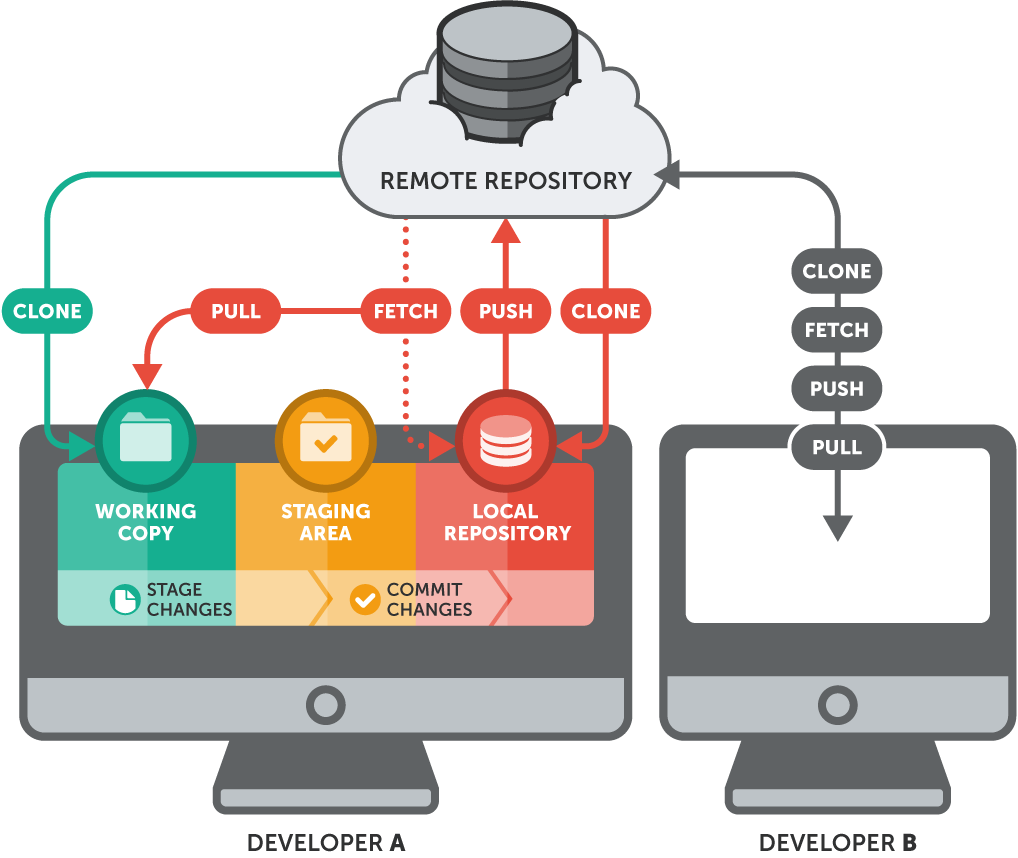
\includegraphics[scale=0.4]{pictures/git.png}
        		\end{center}
        		\legend{Fonte: \url{https://raw.githubusercontent.com/UnbDroid/AprendendoGithub/master/images/git.png}}
        	\end{figure}
        	
        	Para realizar a sincronização entre repositórios locais e remotos o Git possibilita o uso de diversos protocolos de rede, temos entre eles principalmente: HTTP(S), FTP, rsync ou SSH.
        	
        	Durante o processo de uso do Git algumas ações são frequentemente utilizadas, e valem ser destacadas aqui, essas são:
        	\begin{itemize}
            	\item \textbf{git init:} 
            	Inicia um repositório git vazio no diretório.
            	
            	\item \textbf{git clone:}
            	Cria um cópia de um repositório remoto localmente, acaba por fazer um download da estrutura remota para a maquina do usuário.
            	
            	\item \textbf{git fetch:}
        	    Sincroniza o estado do repositório remoto com o local sem realizar alterações na \textit{working tree} do desenvolvedor. Baixa os dados existentes no repositório remote que não existem no computador do usuário.
        	
            	\item \textbf{git checkout:}
            	Alinha o repositório local de acordo com a revisão ou branch especificado no comando.
            	
            	\item \textbf{git commit:}
            	O commit é o ato de criar um ponto no histórico do repositório contendo as mudanças que foram adicionas na área de staging.
            	
            	\item \textbf{git add:}
            	O comando \textit{add} é responsável por adicionar as mudanças especificadas na área de staging do git para serem comitadas em seguida.
            	
            	\item \textbf{git push:}
            	O push executa a ação de enviar os commits locais para o repositório remoto especificado.
            	
            	\item \textbf{git merge:}
            	Atualiza os arquivos na working tree para corresponderem ao especificado no comando. O merge também pode acabar atualizando o HEAD do branch atual.
            	
            	\item \textbf{git pull:}
            	Esse comando realiza a atualização do repositório local a partir das mudanças realizadas no repositório remoto. De forma geral ele acaba realizando um download dos commits mais recentes que estão presentes no remote. É uma combinação do git fetch com o git merge FETCH\_HEAD
        	\end{itemize}
        	\begin{figure}[htb]
        		\caption{\label{fig_git2}Fluxo de trabalho em Git}
        		\begin{center}
        		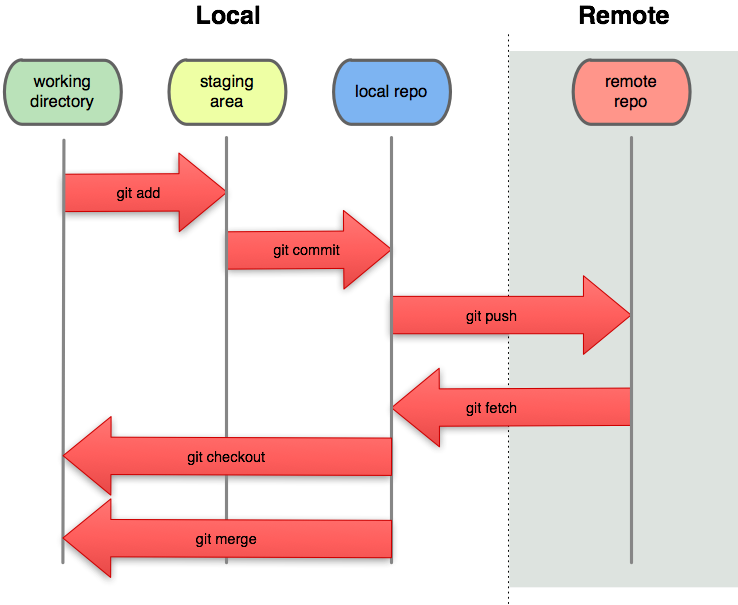
\includegraphics[scale=1]{pictures/GIT2.png}
        		\end{center}
        		\legend{Fonte: \url{https://kevintshoemaker.github.io/StatsChats/GIT2.png}}
        	\end{figure}
        	
    	\subsection{GraphQL}
            GraphQL é uma linguagem de consulta criada pelo Facebook em 2002 e lançada publicamente em 2015. É utilizada principalmente em conjunto com o protocolo HTTP no contexto de um servidor web para que um cliente possa obter os dados que necessita de um servidor.
            Ele tem algumas características que torna seu uso interessante, como por exemplo:
            - Ela permite que o cliente especifique exatamente quais dados ele quer que sejam retornados em determinada requisição
            - Torna fácil o processo de agregação de dados vindos de diferentes fontes.
            - Utiliza um sistema de tipos para descrever dados.
    
            Além disso, a comunidade oferece diversos \textit{Frameworks} que atuam no lado do cliente e que são responsáveis pela obtenção, cacheamento e normalização dos dados. Os mais relevantes são Apollo e Relay (também desenvolvido e mantido pelo Facebook). Do lado do servidor, existe uma infinidade de implementações de GraphQL nas mais diferentes linguagens de programação, sendo a mais popular a implementação de referência em Javascript, mantida pela própria empresa criadora da linguagem.
        
            GraphQL é uma alternativa ao modelo REST e vem ganhando espaço no mercado nos últimos anos, sendo utilizado por grandes empresas como Facebook e Github em seus produtos mais importantes.
    
        \subsection{ZeroMQ} 
        
        ZeroMQ é um biblioteca escrita originalmente em C que provê a ferramentas para a construção de mecanismos de rede embarcada em aplicações diversas. Ela fornece diversos tipos de \textit{sockets} que carregam mensagens atômicas através de diversos protocolos de transporte, como por exemplo TCP. O ZeroMQ possibilita a criação de topologias e padrões de conexão de \textit{sockets} extremamente variáveis e flexíveis, entre eles \textit{fan-out}, \textit{pub-sub}, \textit{request-reply}, entre outros. A implementação do ZeroMQ se utiliza de um modelo de I/O assíncrono que permite fácil escalabilidade e uma grande quantidade de carga. ZeroMQ tem bibliotecas em implementações na grande maioria das linguagens de programação, tornando ele um boa opção para arquiteturas mistas.\cite{zeromqguide}
        
    \section{Linguagens de Programação}
    	\subsection{Clojure}
    	    Clojure é uma linguagem de programação dinâmica e funcional. Sendo um dialeto de LISP que roda na JVM, é uma linguagem compilada, mas que mantém todas características dinâmicas a ser utilizadas em Runtime. Possui compatibilidade e interoperabilidade com todo ecossistema Java e de outras linguagens que rodem na JVM. Clojure enfatiza o uso de estruturas de dados imutáveis e de a filosofia de Code is Data, com um sistema poderoso de macros e de estruturas de dados mutáveis Thread Safe quando necessário. \cite{clojurerationale}
	
    	    Clojure é a principal linguagem de programação utilizada no Nubank, e também é muito familiar para o grupo, além de apresentar características interessantes para o desenvolvimento do projeto. como a grande habilidade para lidar com problemas de concorrência de forma segura e eficiente.
	
	        Dentro do desenvolvimento do projeto Clojure foi utilizada como uma das principais linguagens de programação para serviços de Backend. Um dos recursos que torna Clojure especialmente interessante é a possível interação em tempo real com o código através de um REPL (Read Eval Print Loop), algo que foi utilizado em um dos módulos do projeto como será descrito mais a frente. Além disso a familiaridade dos desenvolvedores do Nubank com a linguagem foi um fator decisivo para que o projeto pudesse continuar a ser mantido por mais pessoas no futuro.
	
        	\begin{figure}
        	    \centering
        	    
\includegraphics[scale=0.1]{pictures/clojure_logo.png}
        	    \caption{Logo Clojure}
        	    \legend{Fonte: \url{https://cdn-images-1.medium.com/max/1200/1*eLqeIits5crU3G5b9LMEyg.png}}
        	    \label{fig:logo_clojure}
        	\end{figure}
	
        \subsection{Javascript} %% TODO: Paps
            Javascript é uma linguagem de programação interpretada baseada em ECMAScript. Foi originalmente criada para atuar junto com navegadores web, tornando possível que scripts fossem executados no lado do cliente sem passar pelo servidor, realizando comunicação assíncrona (AJAX) a manipulando o conteúdo do documento exibido em páginas web.
            
            Ela foi concebida par ser uma linguagem script com orientação a objetos baseada em protótipos, tipagem fraca e dinâmica e funções de primeira classe. Possui suporte à programação funcional e apresenta recursos como \textit{Closures} e \textit{higher-order functions}.

            Hoje é uma das linguagens mais populares do mundo e já há alguns anos vem sendo bastante utilizada no lado do servidor através de ambientes como Node.js. 
	
	
            \subsubsection{Typescript}
                Typescript é uma linguagem de programação desenvolvida e mantida pela Microsoft que tem como objetivo tornar bases de código em Javascript mais fáceis de se manter e menos suscetíveis à erros, através da adição de um sistema de tipos à linguagem, entre outros recursos. 

                Para que o código escrito em Typescript possa de fato ser executado em ambientes como navegadores web e Node.js, é preciso compilá-lo para Javascript e este processo pode ser feito através do compilador oferecido como parte do ferramental da linguagem. Na verdade, todo código Javascript é um código Typescript válido, porém o contrário não é verdadeiro.

            \subsubsection{Node.js}
                Node.js é um ambiente de execução multiplataforma e de código aberto, com a capacidade de executar Javascript fora do contexto de um browser, tornando possível o uso da linguagem em um ambiente de servidor.
    
                Utiliza o motor de Javascript V8, desenvolvido pela Google e que está presente também em seu navegador Google Chrome. Node.js segue uma arquitetura \textit{event-driven} capaz de realizar I/O de maneira assíncrona e não bloqueante. Estas escolhas de projeto tem como objetivo otimizar o \textit{throughput} e escalabilidade em aplicações web com muitas operações de entrada e saída, bem como aplicações web \textit{real-time} como por exemplo programas de comunicação em tempo real e jogos.

                Como parte de seu ecossistema, é oferecido um gerenciador de pacotes chamado \textit{npm}, que conta com uma interface de linha de comando e um banco de dados público de pacotes, que podem ser adicionados em projetos através de um sistema de dependência.

                Hoje Node.js é utilizado por empresas como GoDaddy, Groupon, IBM, Linkedin, Microsoft, Netflix, PayPal, Rakuten, Walmart, Yahoo, entre outros.

    \section{React}
        React é uma biblioteca JavaScript de código aberto para criar interfaces interativas. É declarativa, eficiente e flexível e permite que o desenvolvedor componha interfaces complexas a partir de partes menores e isoladas chamadas "componentes".

        Utiliza a técnica de \textit{Virtual DOM}, o que melhora drasticamente sua performance pois diminui o número de operações feitas de fato no DOM (\textit{Document Object Model}), que costumam ser tarefas de processamento mais intensivo.

	
	\section{Docker}
	    Docker é uma plataforma \textit{open source} para desenvolvimento de aplicações através de contêineres, criada e mantida pela empresa Docker Inc. Foi escrito na linguagem de programação Go, que é fortemente tipada e possui \textit{garbage collector} para gerenciamento de memória, além de suporte explícito para programação concorrente.
	
	    No seu ecossistema existem ferramentas para criação de imagens e execução de con\-têi\-ne\-res (\textit{Docker Engine}), repositórios para distribuição de imagens (\textit{Registries}) e também uma ferramenta para orquestração de con\-têi\-ne\-res em um cluster (\textit{Docker Swarm})
	
	
    	\subsection{Base tecnológica}
    	    O Docker se utiliza de diversos recursos do kernel do sistema operacional para prover a tecnologia de contêineres, como \textit{cgroups}, que permitem que os processos sejam organizados em grupos hierárquicos e cuja utilização de recursos pode ser limitada e monitorada. \textit{Namespaces}, que permitem que um sistema isole uma coleção de processos para que não possam ver certas partes do sistema geral e o \textit{Unionfs}, que é um sistema de arquivos empilhável que permite aos usuários especificar um conjunto de diretórios que são apresentados como um único diretório virtual, mesmo que estes possam vir de diferentes sistemas de arquivos.
    	
    	\subsection{Arquitetura}
    	    Utiliza-se de uma arquitetura cliente-servidor composta por três componentes: um \textit{Daemon}, que é o responsável por criar e manipular os objetos Docker (imagens, contêineres, redes, volumes, \textit{etc.}) e age como servidor.
    	
    	    Uma API REST, que define uma interface que os outros programas podem utilizar para interagir com o daemon e instruí-lo sobre o que fazer.
    	
    	    Uma interface de linha de comando, que é a principal interface do usuário com o Docker. Ela age como cliente e se utiliza da API REST para interagir com o daemon através de scripts ou diretamente de comandos em um terminal.
    	
    	\subsection{Objetos Docker}
    	    \subsubsection{Imagens}
    	        Uma imagem é um \textit{template read-only} com instruções para a criação de um contêiner Docker. Normalmente é baseada em outra imagem, com customizações adicionais. Por exemplo, é possível construir uma imagem baseada na imagem do \texttt{ubuntu}, porém que instala e configura um servidor web Apache e uma determinada aplicação.
    	
    	        Para criar uma imagem, é preciso um Dockerfile, arquivo que se utiliza de uma sintaxe simples para definir os passos necessários para criar a imagem e executá-la. Cada instrução em um Dockerfile cria uma camada na imagem, que são reaproveitadas quando a imagem é reconstruída caso a instrução continue a mesma. Esta estratégia é responsável por tornar as imagens leves e rápidas, quando comparadas com outras tecnologias de virtualização.
    	
        	\subsubsection{Contêineres}
        	    Um contêiner é uma instância executável de uma imagem. É possível criar, pausar, interromper, mover e remover um contêiner utilizando a interface de linha de comando ou a API REST. É possível também conectar um contêiner em uma ou mais redes, acoplar volumes de dados ou mesmo gerar novas imagens a partir do estado atual de um contêiner.
        	
    	        Por padrão, um contêiner é relativamente bem isolado de outros contêineres e da máquina hospedeira, e este nível de isolamento pode ser controlado através dos mecanismos de redes e volumes oferecidos pelo Docker.
    	
    	        Um contêiner é efêmero do ponto de vista que nenhuma das mudanças em seu estado que não forem armazenadas de maneira persistentes serão perdidas assim que o contêiner é removido. \cite{dockeroverview}
	
	
	\section{Kubernetes}
	    Kubernetes é um projeto de código aberto da Google, que possui mais de 1800 contribuidores e ganha cada vez mais atenção no mundo de operação e desenvolvimento de software. 
	    A Google, dado a escala de sua operação, sofria com problemas com o gerenciamento de muitas máquinas virtuais. 
    	Assim, precisou-se repensar como lidar com esse problema, o que, depois de anos, levou ao gerenciador e escalonador de contêineres chamado Kubernetes.

    	Para entender melhor a necessidade de um gerenciador tal como o Kubernetes, é necessário dar um passo atrás e olhar para as vantagens e desvantagens dos contêineres.
    	Contêiners são feitos para serem leves, rápidos, mas de duração curta e frágeis.
    	Assim, eles trocaram a resiliência de uma máquina virtual pela velocidade e leveza. Isso requer que contêineres rodem em um ambiente onde em caso de falha ou mudança de carga, esse ambiente garanta a substituição desses contêineres e gerencie eventuais mudanças de rede e recursos de memória e CPU do \textit{cluster}.
    	
    	Kubernetes trabalha com a ideia de guardar o estado desejado do \textit{cluster}. Isso porque, em sistemas distribuídos, é importante a construção de um modelo de estado global.\cite{globalstate} Muitos problemas são resolvidos com uma boa modelagem de estado global. Para isso, o Kubernetes provê alguns objetos através da sua API. Dentre todos os objetos, os relevantes para o nosso projeto são:
    	
	    \begin{itemize}
	        \item \textit{Namespace}: provêm um escopo de nomes, são projetados para ambientes nos quais há diversos usuários do \textit{cluster}. Recursos dentro de um namespace devem ter um nome único.\cite{k8sdocsnamespace}
	        \item \textit{Pod}: respresenta a unidade mais simples capaz de ser distribuída pelo Kubernetes. É o bloco básico para construção de outros objetos. Encapsulam um ou mais contêineres que representam uma aplicação, com todos os requisitos de disco e rede. Pods são efêmeros, isto é, eles podem ser removidos e recriados sem aviso prévio. \cite{k8sdocspods}
	        \item \textit{Deployment}: é um dos objetos controladores, provém atualizações declarativas aos \textit{Pods}. Capaz de criar e gerenciar réplicas de Pods, \textit{rollout} de atualizações, reinício de \textit{Pods} em caso de falha. \cite{k8sdocsdeployments}
	        \item \textit{Service}: é uma abstração que define um conjunto lógico de \textit{Pods} e uma política de acesso a ele.\cite{k8sdocsservice} Quando um \textit{Service} é criado dentro de um \textit{Namespace}, é criado uma entrada de DNS, permitindo que os \textit{Pods} se encontrem na rede apenas pelo nome do \textit{Service}, garantindo que com a mesma configuração, serviços acessem recursos de seus respectivos \textit{Namespaces}. \cite{k8sdocsnamespace}
	        \item \textit{Ingress}: são configurações de acesso externo ao \textit{cluster}, tipicamente HTTP. \cite{k8sdocsingress} 
	    \end{itemize}
